\section{Preliminaries}
\label{preliminary}

\subsection{Notations}
In our problem, we consider a network modeled as a graph $G = (V,E)$, which represents a vertex set $V$ and edge set $E$. For a source node $s$ and a target node $t$, we are interested in finding a path $p(s,t)=(s,v_1,v_2,...,v_{l-1},t)$ with a length of $|p(s,t)|$ close to the exact distance between $s$ and $t$ in the graph. Let $P(s,t)$ be the set of all paths from s to t. We can then define the distance between $s$ and $t$ as $d_G(s,t) = min_{p(s,t) \in P(s,t)}|p(s,t)|$.

\subsection{Problem formulation}

Our problem formulation is as follows: given a graph $G$, construct an index structure, and perform decentralized search based on the index to answer approximate shortest path queries of arbitrary pair of vertices in large scale networks. We are focusing on a specific kind of networks which is very common in real-world networks called the complex networks.

We will focus on unweighted, undirected graphs in this paper. But all the ideas presented in this paper can be extended for weighted and/or directed graphs.

\subsection{Landmark based indexes}

\begin{figure}[t]
    \centering
    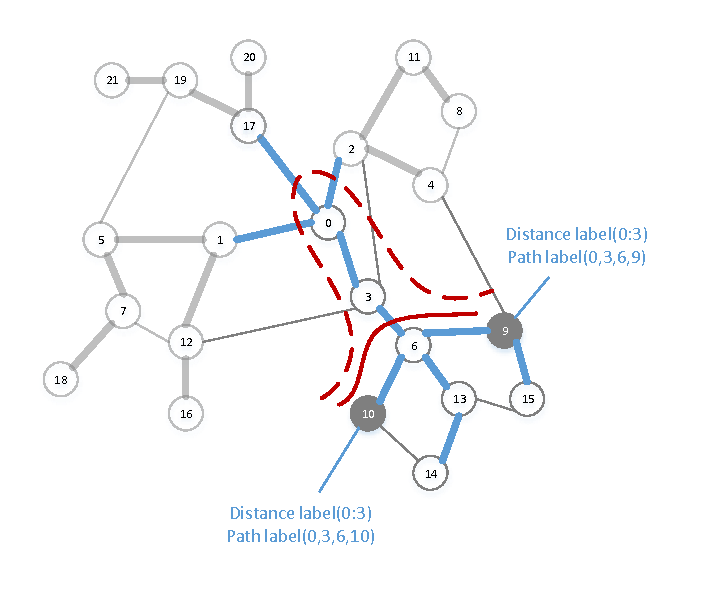
\includegraphics[width=\linewidth]{../figures/new_illustrate/basic_lca.pdf}
    \caption{Distance of path estimated by distance-only label and path label. The dashed curved line shows the path estimated by the distance-only label. The solid curved line shows the path estimated by the path label.}
    \label{fig:basic_lca}
\end{figure}

Our method is motivated by the idea of using landmarks as the basis for indexes. Specifically, given a graph $G$ and a small (constant) set of landmarks $L$, $|L|$ BFS traversals are needed to compute shortest paths between each vertex in $G$ to each landmark in $L$. An index for the graph is constructed such that it contains a label $L(v)$ for each vertex. Each label can store either the distance to each landmark $(l_i, d_G(v,l_i))$ or the shortest path to each landmark $(l_i, p(v,l_i))$ where $|p(v,l_i)| = d_G(v,l_i)$.

Since the shortest-path distance satisfies the triangle inequality, for an arbitrary pair of vertices $s$ and $t$, we have the following bounds:

\begin{equation}
\label{equ:upper}
    d_G(s,t) \leq min_{l \in L}\{d_G(s,l) + d_G(l,t)\}
\end{equation}
\begin{equation}
\label{equ:lower}
    d_G(s,t) \geq max_{l \in L}|d_G(s,l) - d_G(l,t)|
\end{equation}

Usually the upper bound can be used as an approximation of the distance of $s$ and $t$. Note that if $s$ and $t$ are not connected with each other, there will not be a common $l$ from $L(s)$ and $L(t)$.

\subsection{The least common ancestor distance}

By indexing the shortest paths instead of distances into the label, one can not only derive an estimated path directly from labels of source and target vertices, but also have a better accuracy with the estimated distance. For example, in Fig. \ref{fig:basic_lca}, the distance estimated from distance-only labels of vertex $9$ and $10$ is 6, representing the length of path $(9, 6, 3, 0, 3, 6, 10)$ shown in the dashed curved line. Although there is a clearly shorter path $(9, 6, 10)$ shown in solid curved line, with distance-only labels, such a path cannot be found. 

More formally, we call the vertex $6$ in the previous example as a common ancestor of vertex $9$ and $10$. When shortest paths rather than distances have been indexed, to get better accuracy, the common ancestors closest to the source and target should be derived from the labels first. This common ancestor is called the least common ancestor $c_l(s,t)$ of the source and target vertex. Then instead of calculating upper bounds from the landmark $l$, the least common ancestor is used:

\begin{equation}
\label{equ:lca}
    d_G(s,t) \leq min_{l \in L}\{d_G(s,c_l(s,t)) + d_G(c_l(s,t),t)\}
\end{equation}

We refer to this upper bound as LCA distance $d_{LCA}(s,t)$ in this paper, which is a more accurate estimation of distance of source and target vertices. Note that both LCA distance and related paths can be derived directly from labels. For example, the path $(9,6,10)$ can be directly derived from the labels of the vertex $9$:$(0:(0,3,6,9))$ and the vertex $10$:$(0:(0,3,6,10))$ by combining the path from source vertex to LCA $(9,6)$ and the path from LCA to target vertex $(6,10)$.
